% =====================================================================
%  ZipCount -- TASLP / journal version (no hard page limit)
%  Compile: pdflatex main_taslp && bibtex main_taslp && pdflatex x2
%  Needs: texlive-publishers (IEEEtran), texlive-pictures (tikz)
%  Companion short version: main_icassp.tex
% =====================================================================
\documentclass[journal]{IEEEtran}

\usepackage{amsmath,amssymb}
\usepackage{booktabs}
\usepackage{multirow}
\usepackage{tikz}
\usetikzlibrary{arrows.meta,positioning}
\usepackage[hidelinks]{hyperref}

\newcommand{\best}[1]{\textbf{#1}}
\newcommand{\sys}{ZipCount}

\begin{document}

\title{Low-Latency Streaming Speaker Counting\\with a Frozen ASR Encoder}
\author{Anonymous Submission}
\markboth{IEEE/ACM Transactions on Audio, Speech, and Language Processing}%
{Anonymous: Low-Latency Streaming Speaker Counting}
\maketitle

\begin{abstract}
Frame-level speaker counting -- how many people are talking at each instant
-- underpins overlap-aware transcription, meeting analytics and turn-taking
control, but is usually obtained as a by-product of speaker diarization
systems that are offline or operate at multi-second latency. We present
\sys{}, a streaming counter that emits a 4-way ordinal count
$\{0,1,2,3^{+}\}$ every $640$\,ms with no lookahead, built by freezing a
public streaming Zipformer ASR encoder and training only a
$1.28$\,M-parameter causal decoder -- $2\%$ of the $65.8$\,M total. A
multi-scale hypercolumn over the encoder's U-shaped stacks, a dev-selected
fixed stack mask with a learned gated projection and a dual-dilation
temporal convolutional decoder supply the segment-scale context counting
requires while remaining strictly causal. Because published speaker-counting
numbers are rarely comparable, we re-score six system configurations under a
single protocol -- identical windows, identical $100$\,Hz ground-truth
rasterization, a common-window restriction -- across four corpora, and
report \sys{} as the mean of 3 independently trained seeds (per-seed
standard deviation $0.002$). At $640$\,ms latency \sys{} comes within
$0.004$ mean macro-F1 of NVIDIA's Sortformer-streaming running at its own
$15.1$\,s default budget, and exceeds it by $0.028$ at matched latency, an
offline Sortformer by $0.014$ and pyannote.audio~3.1 by $0.040$. A heavier
offline WavLM
pipeline remains clearly ahead, and we report in full the one corpus where
\sys{} ranks last. We additionally document a set of negative results:
eight candidate architectural and loss components that did not survive
paired testing, a measured ceiling showing that only $\approx\!20\%$ of the
gap to the strongest baseline is attributable to the causal constraint, and
seed-structural instability under encoder fine-tuning. \sys{} runs at
$\mathrm{RTF}=0.032$ on GPU and $0.080$ single-threaded on CPU.
\end{abstract}

\begin{IEEEkeywords}
speaker counting, overlapped speech detection, streaming speech processing,
speaker diarization, frozen encoders, transfer learning
\end{IEEEkeywords}

% =====================================================================
\section{Introduction}
\IEEEPARstart{K}{nowing} how many speakers are active in each frame is a
compact but consequential signal. It gates overlap-aware ASR, drives
barge-in and turn-taking logic in conversational agents, and is the quantity
that overlapped speech detection (OSD) reports in binary form. Unlike full
diarization it requires no speaker identity, no clustering and no bounded
speaker inventory, which makes it a natural fit for streaming deployment.

In practice, however, counting is usually read off a diarization system.
Clustering pipelines such as pyannote.audio~\cite{bredin2023pyannote} and
WavLM-based systems~\cite{han2024diarizen,chen2022wavlm} are offline by
construction: they embed and cluster the whole recording. End-to-end neural
diarization (EEND)~\cite{fujita2019eend} and its streaming
descendants~\cite{liang2024fseend,liang2025lseend} relax this, and NVIDIA's
Sortformer~\cite{park2024sortformer} ships an explicitly streaming
checkpoint -- but, as we measure in Section~\ref{sec:results}, its default
operating point carries an algorithmic latency of $15.1$\,s. ``Streaming''
there means bounded memory over long recordings, not real-time response.

We take the opposite starting point: fix the latency budget first at
$640$\,ms with zero lookahead, then ask how much counting accuracy is
attainable within it. Our answer reuses a frozen streaming ASR encoder.
Speech recognition encoders already resolve overlapping talkers as an
obstacle to be modelled, and streaming ASR encoders are trained under
exactly the causal constraint we need. Keeping the encoder frozen makes the
system cheap to train and, as Section~\ref{sec:negative} shows, markedly
more stable than fine-tuning it.

Our contributions are:
\begin{enumerate}
\item A $640$\,ms-latency streaming speaker counter combining a frozen
streaming Zipformer~\cite{yao2024zipformer} with a multi-scale hypercolumn,
a dev-selected fixed stack mask with a learned gated projection, and a
causal dual-dilation TCN decoder (Section~\ref{sec:method}).
\item A unified re-scoring protocol for speaker counting
(Section~\ref{sec:protocol}): window length and frame rate silently change
macro-F1, so we re-run six system configurations on identical assets, and
report \sys{} as a mean over 3 independently trained seeds rather than a
single checkpoint.
\item A four-corpus evaluation (Section~\ref{sec:results}) with per-class
scores, DER context and measured real-time factors, including an explicit
account of which evaluation material is in-domain for which system.
\item A documented set of negative results (Section~\ref{sec:negative}):
eight rejected components, a context-oracle measurement bounding how much of
the remaining gap causality explains, and fine-tuning instability that lower
learning rates do not remove.
\end{enumerate}

% =====================================================================
\section{Related Work}

\textbf{Counting and overlap detection.} Frame-level speaker counting is
closely related to OSD, where TCN-based detectors over meeting corpora are
established practice~\cite{cornell2020osd,bullock2020overlap}. Real-time
single-channel counting has also been addressed
directly~\cite{yousefi2021realtime}. These systems are typically non-causal,
binary ($\geq\!2$ speakers), or both; we predict a 4-way ordinal count
causally and evaluate OSD as a derived $c\!\geq\!2$ view of the same output,
which keeps the two tasks on one head rather than two models.

\textbf{Streaming diarization.} FS-EEND~\cite{liang2024fseend} and
LS-EEND~\cite{liang2025lseend} perform frame-online EEND with attractors,
the latter recovering a speaker count through a termination marker.
Sortformer~\cite{park2024sortformer} reformulates diarization with a sorted
objective and provides a streaming variant built on a speaker cache and FIFO
queue. We benchmark against the released streaming checkpoint at both its
default latency and, explicitly off-label, at our own $640$\,ms budget.

\textbf{Frozen encoders with light heads.} Reusing a frozen self-supervised
or ASR encoder under a small task head is now common, including for speaker
attribution on top of frozen ASR models~\cite{msaasr2024}. Our contribution
is not the pattern but its instantiation under a hard causal latency
constraint, together with the finding (Section~\ref{sec:ablation}) that
\emph{which} encoder scales are exposed to the head matters more than head
capacity.

% =====================================================================
\section{Method}
\label{sec:method}

\begin{figure}[t]
\centering
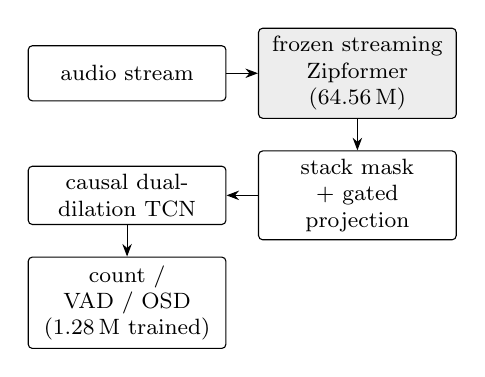
\begin{tikzpicture}[
  font=\footnotesize,
  box/.style={draw,rounded corners=1.5pt,align=center,inner sep=3pt,
              minimum height=7mm,text width=23mm},
  ar/.style={-{Stealth[length=1.6mm]}}]
\node[box] (a) {audio stream};
\node[box,right=4mm of a,fill=black!7] (z) {frozen streaming\\Zipformer\\(64.56\,M)};
\node[box,below=4mm of z] (s) {stack mask\\+ gated projection};
\node[box,left=4mm of s] (t) {causal dual-\\dilation TCN};
\node[box,below=4mm of t] (h) {count / VAD / OSD\\(1.28\,M trained)};
\draw[ar] (a)--(z); \draw[ar] (z)--(s); \draw[ar] (s)--(t); \draw[ar] (t)--(h);
\end{tikzpicture}
\caption{System overview. The encoder is frozen; only the gated projection,
TCN decoder and output head are trained ($2\%$ of parameters). Output is
$25$\,Hz, emitted in blocks of $16$ frames every $640$\,ms.}
\label{fig:arch}
\end{figure}

\subsection{Task and latency accounting}
Given a causal audio stream, the model emits at $25$\,Hz a distribution over
$c_t \in \{0,1,2,3^{+}\}$, the number of simultaneously active speakers in
frame $t$. Inference proceeds in blocks of $16$ output frames, one per
$640$\,ms, with no right context.

Because a chunked emitter does not delay every frame equally, we state the
budget component-wise. Lookahead is $0$\,ms. Within a block, frame $i$ waits
$640 - 40i$\,ms for its block to complete, so the chunking delay is
$640$\,ms worst-case (first frame) and $340$\,ms averaged over the block.
Compute adds $20.7$\,ms (Section~\ref{sec:results}), giving a worst-case
end-to-end response of $660.7$\,ms. We use ``$640$\,ms latency'' throughout
as shorthand for the worst-case chunking budget.

\subsection{Frozen streaming backbone}
The backbone is the public LibriSpeech streaming
Zipformer~\cite{yao2024zipformer} ($64.56$\,M parameters), used causally
with chunk size $32$ and $128$ left-context frames, and entirely frozen.
The chunk size is counted in the encoder's $50$\,Hz embedding frames, so
$32$ frames is exactly $640$\,ms of newly received audio; the encoder
internally downsamples by $2\times$ to the model's $25$\,Hz output rate,
yielding the $16$-frame output block referenced throughout this paper.
Zipformer's encoder is U-shaped: six stacks with downsampling factors
$(1,2,4,8,4,2)$ and widths $(192,256,384,512,384,256)$ operate at different
temporal resolutions, which is precisely the property we exploit.

\subsection{Multi-scale hypercolumn and stack selection}
\label{sec:hypercolumn}
Rather than consume only the final stack, we form a hypercolumn by
resampling every stack to the common $25$\,Hz output rate and concatenating,
giving a $1984$-dimensional per-frame descriptor. A gated projection
LayerNorm-izes each stack slice separately -- their activation scales differ
by an order of magnitude -- weights the slices by a softmax gate, and
projects to $d\!=\!192$.

We additionally apply a fixed binary stack-selection mask
$m \in \{0,1\}^{6}$. A masked slice is replaced by an exact zero block
\emph{after} its LayerNorm and \emph{before} the gate, so no masked feature
can reach the output, while every module -- and hence the parameter count,
the state-dict keys and the seeded initialization -- remains identical
across mask settings. Mask ablations are therefore parameter- and
initialization-matched by construction, which matters because the effects we
measure are of the order of the seed noise.

The softmax gate is deliberately \emph{not} renormalized over the active
subset. Masked gates still absorb probability mass -- in our trained model
$0.57$ of it, distributed equally over the three masked stacks, since their
zeroed features admit gradient only through the softmax denominator -- but
because they multiply zero blocks this acts purely as a global rescaling of
the fused vector, which the immediately following linear projection absorbs
column-wise. Renormalizing changes optimization dynamics, not the model
class. Our main system uses $m=(1,1,1,0,0,0)$, i.e.\ the three
highest-time-resolution stacks.

\subsection{Causal dual-dilation TCN decoder}
An overlap is confirmed by seconds of evidence, but its boundaries are
frame-local. The decoder therefore stacks six residual blocks with dilations
$1,2,4,8,16,32$; each block runs \emph{two} depthwise convolutions
(kernel $3$) over the same normalized input -- one at dilation $1$ for
onset/offset detail, one at dilation $d$ for segment-scale context --
concatenates them and passes the result through a GLU, so the block gates
context against detail per frame. Padding is left-only, giving a receptive
field of $127$ frames ($5.08$\,s of past) with strict causality, which we
verify by asserting that a future-frame perturbation cannot change past
outputs.

For streaming, each block caches its last $(k\!-\!1)d$ \emph{post}%
-normalization frames. This matters only at stream start, but it matters
concretely: \texttt{forward} pads after the LayerNorm, so the initial cache
must be literal zeros, whereas prepending raw zeros before the norm yields
the LayerNorm bias $\beta$ instead. In trained checkpoints
$|\beta| \in [0.057, 0.092]$, which perturbs the first receptive field of
every stream by up to $0.014$ logit -- invisible to an equivalence test on a
freshly initialized head, where $\beta = 0$.

\subsection{Ordinal-consistent output and objective}
\label{sec:objective}
The head emits 4-way count logits and, from the same trunk, two cumulative
logits $P(c\!\geq\!1)$ (VAD) and $P(c\!\geq\!2)$ (OSD). Training ties the
two views together with consistency and monotonicity terms, so the ordinal
structure of the label is exploited without giving up the softmax view that
works best for overlap. The decoder and head together contain $1.28$\,M
parameters, the only trainable weights in the system.

The objective is
\begin{equation}
\mathcal{L}=\mathcal{L}^{\text{SORD}}_{\text{count}}
+\lambda_{\text{aux}}^{\top}\mathcal{L}_{\text{aux}}
+\lambda_{\text{reg}}^{\top}\mathcal{L}_{\text{reg}} .
\end{equation}
$\mathcal{L}^{\text{SORD}}$ uses soft ordinal labels~\cite{diaz2019sord}
($\alpha\!=\!2.5$) with class weights $(1,1,1.5,3)$ offsetting the rarity of
classes $2$ and $3^{+}$. $\mathcal{L}_{\text{aux}}$ collects binary VAD
($0.3$), overlap ($0.5$), Dice ($0.5$), branch consistency ($0.2$) and
monotonicity ($0.1$); $\mathcal{L}_{\text{reg}}$ collects an expected-MAE
term exploiting ordinality ($0.2$) and a symmetric-KL temporal smoothness
term ($0.02$).

% =====================================================================
\section{Experimental Setup}

\subsection{Training data and schedule}
The head is trained for $3000$ steps (batch $24$, Adam, lr $10^{-3}$ cosine
with $500$ warmup steps, AMP) on $253{,}452$ $30$-second windows drawn from
LibriMix~\cite{cosentino2020librimix} 2- and 3-speaker mixtures
($107{,}900$), AMI~\cite{carletta2005ami} ($39{,}464$), NOTSOFAR-1
($32{,}432$), AliMeeting ($26{,}868$), AISHELL-4 ($11{,}723$),
MSDWild~\cite{liu2022msdwild} ($8{,}558$), RAMC ($6{,}000$),
VoxConverse~\cite{chung2020voxconverse} ($2{,}507$), plus single-speaker,
MUSAN-noise~\cite{snyder2015musan} and silence windows. MUSAN noise
($p\!=\!0.5$, $0$--$20$\,dB SNR), simulated RIRs ($p\!=\!0.8$) and gain
jitter are applied to the synthetic portion only; real meeting corpora are
left unaugmented as they already carry room acoustics. At batch $24$ this
schedule presents $72{,}000$ windows, i.e.\ under one third of an epoch;
we fixed the endpoint before the architecture search and never re-tuned it,
which is what makes the paired comparisons in Section~\ref{sec:negative}
interpretable.

Training and test splits are disjoint, but we stress that AMI, VoxConverse
and MSDWild are \emph{in-domain} for \sys{} -- their training splits are in
the mix -- while DipCo~\cite{vansegbroeck2020dipco} is never seen. The
baselines have their own, differently overlapping training data; no system
in Table~\ref{tab:main} is domain-neutral, and we interpret results
accordingly.

\subsection{Unified evaluation protocol}
\label{sec:protocol}
Speaker-counting numbers are highly sensitive to two choices that are
frequently left implicit. The first is the \emph{window length} presented to
the system, which determines how much context an offline model receives. The
second is the \emph{frame rate} at which predictions and references are
rasterized, which determines how boundary frames are charged. Comparing a
system scored on $30$\,s windows at $25$\,Hz against one scored on $90$\,s
windows at $100$\,Hz is not meaningful, yet the two numbers look directly
comparable, and in our own earlier work they were compared.

We therefore re-score \emph{every} system, including our own, on identical
assets: $90$\,s windows cut from the original per-speaker RTTM ground truth,
rasterized at $100$\,Hz. \sys{}'s $25$\,Hz predictions are upsampled
$4\times$, which charges it honestly for the $40$\,ms boundaries it cannot
place. Since one baseline fails on a small number of short windows, all
systems are additionally restricted to the common set of windows every
system produced output for ($570$/$583$ on AMI, complete on DipCo and
MSDWild). For VoxConverse and MSDWild, which lack the manifest format our
asset builder originally required, we built assets directly from the
corpora's official RTTM files and verified window offset re-basing by hand
against the source annotations. Diarization outputs are converted to counts
by summing active speaker tracks per frame, using the same rasterizer for
every system.

\subsection{Model selection and the development set}
\label{sec:selection}
Every architecture decision reported here -- the decoder choice, the stack
mask, and the eight further candidate components of
Section~\ref{sec:negative} -- was made on a single fixed development set: a
$116$-recording half of the VoxConverse test set, which we call
\emph{vox-sel}. Loss weights and the $3000$-step endpoint were fixed before
that search began and never re-tuned. No AMI, DipCo or MSDWild material was
ever inspected during selection, so those three columns of
Table~\ref{tab:main} are untouched by it.

VoxConverse itself is not, and we therefore exclude the development half
from all reported numbers, scoring the VoxConverse column only on the sealed
complementary half (\emph{vox-lock}, $116$ recordings, $964$ windows). The
difference is measurable and we report it rather than absorb it: moving from
the development half to the sealed half costs \sys{} $0.021$ macro-F1
($0.560\!\rightarrow\!0.539$), the largest shift of any system, while the
five baselines -- none of which were tuned on either half -- move by
$-0.013$ to $+0.024$ (Table~\ref{tab:leak}). Since the two halves evidently
differ somewhat in intrinsic difficulty, $0.021$ should be read as an upper
bound on the selection penalty rather than a clean estimate of it. A
single-corpus development set is a real limitation of this study.

\begin{table}[t]
\centering
\caption{Macro-F1 on the development half (\emph{vox-sel}) versus the sealed
half (\emph{vox-lock}) of VoxConverse. Only \sys{} was tuned on
\emph{vox-sel}.}
\label{tab:leak}
\small
\begin{tabular}{lccc}
\toprule
System & vox-sel & vox-lock & $\Delta$ \\
\midrule
DiariZen                     & 0.660 & 0.656 & $-0.004$ \\
Sortformer-offline           & 0.628 & 0.624 & $-0.004$ \\
Sortformer-str.\ (default)   & 0.656 & 0.680 & $+0.024$ \\
Sortformer-str.\ ($640$\,ms) & 0.607 & 0.616 & $+0.009$ \\
pyannote.audio 3.1           & 0.587 & 0.574 & $-0.013$ \\
\midrule
\sys{} (tuned here)          & 0.560 & 0.539 & $\mathbf{-0.021}$ \\
\bottomrule
\end{tabular}
\end{table}

\subsection{Systems compared}
\textbf{DiariZen}~\cite{han2024diarizen}: WavLM-Large + clustering, offline.
\textbf{Sortformer-offline}~\cite{park2024sortformer}:
\texttt{diar\_sortformer\_4spk-v1}, full utterance.
\textbf{Sortformer-streaming}: \texttt{diar\_streaming\_sortformer\_4spk-v2.1}
at (i) its released default (chunk $188$, right context $1$; algorithmic
latency $15{,}120$\,ms) and (ii) chunk $8$, right context $0$, giving
exactly $640$\,ms. Configuration (ii) is \emph{off-label} -- below the
model's trained operating point -- and we report it as a latency-matched
reference, not as a vendor-recommended setting.
\textbf{pyannote.audio 3.1}~\cite{bredin2023pyannote}: offline; we take the
overlap-preserving output, as the exclusive variant deliberately drops
overlapping speech and would undercount by construction.

\subsection{Metrics}
Our primary metric is macro-F1 over the four count classes, which weights
the rare $2$ and $3^{+}$ classes equally with silence and single-speaker
frames. We report per-class F1 and OSD F1 alongside it, and DER (collar
$0.25$\,s, overlap included) for the five systems that emit speaker
identity. For the ablations we add segmental edit score and fragmentation
rate, borrowed from temporal action segmentation, plus expected calibration
error and Brier score.

% =====================================================================
\section{Results}
\label{sec:results}

\begin{table*}[t]
\centering
\caption{Macro-F1 under the unified protocol. Corpora are weighted equally
in the mean. The VoxConverse column uses only the sealed half of the test
set (Section~\ref{sec:selection}). $^{\dagger}$in-domain for \sys{}
(training split in its mix); DipCo is unseen. $^{*}$off-label
configuration. $^{\ddagger}$\sys{} rows are the mean of 3 independently
trained seeds (1234, 2345, 3456; identical config, different init and
data order), pooled over recordings before scoring; per-seed 4-corpus-mean
std is $0.002$ (Section~\ref{sec:results}).}
\label{tab:main}
\begin{tabular}{lccccc c}
\toprule
System & Latency & AMI-SDM$^{\dagger}$ & DipCo & VoxConverse$^{\dagger}$ & MSDWild$^{\dagger}$ & Mean \\
       &         & (570 win.) & (107 win.) & (964 win.) & (268 win.) & \\
\midrule
DiariZen (WavLM + clustering)      & offline      & \best{0.765} & 0.495 & 0.656 & \best{0.642} & \best{0.640} \\
Sortformer-streaming (default)     & 15{,}120\,ms & 0.564 & 0.518 & \best{0.680} & 0.554 & 0.579 \\
\sys{} (ours)$^{\ddagger}$         & \best{640\,ms} & 0.654 & \best{0.552} & 0.542 & 0.553 & 0.575 \\
Sortformer-offline                 & offline      & 0.606 & 0.501 & 0.624 & 0.513 & 0.561 \\
Sortformer-streaming$^{*}$         & 640\,ms      & 0.539 & 0.495 & 0.616 & 0.537 & 0.547 \\
pyannote.audio 3.1                 & offline      & 0.594 & 0.464 & 0.574 & 0.509 & 0.535 \\
\bottomrule
\end{tabular}
\end{table*}

\subsection{Cross-corpus comparison}
Table~\ref{tab:main} gives the main result. Read by mean macro-F1, DiariZen
is the clear winner ($0.640$), ahead of every other system by more than
$0.06$. \sys{} reaches $0.575$ against Sortformer-streaming's $0.579$ at its
default setting; this is the mean over 3 independently trained seeds, with
seed-to-seed standard deviation $0.002$ (measured directly, not assumed --
see below), so the ranking does not depend on which seed happened to be
reported.

The meaningful comparison is on the latency axis. \sys{} comes within
$0.004$ of Sortformer-streaming while operating at $1/23$ of its latency
budget, and at equal $640$\,ms latency it is ahead by $0.028$. It also
exceeds Sortformer-offline and pyannote.audio, both of which consume the
entire utterance. Against DiariZen the gap is real and we do not minimize
it: a frozen $1.28$\,M-parameter causal head does not replace a fine-tuned
WavLM-Large pipeline with global clustering.

To test these differences rather than merely state them, we run a paired
bootstrap that resamples \emph{recordings within each corpus} and averages
macro-F1 over corpora with equal weight, reproducing exactly the quantity
in Table~\ref{tab:main} ($10{,}000$ resamples; \sys{}'s per-window
confusions are pooled over the same 3 seeds as Table~\ref{tab:main} before
resampling). Recordings are the resampling unit because windows from one
recording share speakers, room and noise conditions and are therefore not
independent draws. We stress that this measures the sampling variance of
the \emph{difference between two fixed systems on this test set}, a
different quantity from the seed-to-seed variance of retraining \sys{}
itself. We measured that variance directly rather than assume it: across
the same 3 seeds, the 4-corpus-mean macro-F1 has standard deviation
$0.002$ (Section~\ref{sec:results}), an order of magnitude below every
resolved gap in Table~\ref{tab:boot} except the Sortformer-streaming-default
comparison, which the bootstrap already reports as unresolved on its own
terms. Conflating this seed variance with the recording-sampling variance
below would still be a category error even though both happen to be small
here.

Table~\ref{tab:boot} gives the result, and it sharpens the latency argument
considerably. The gap to Sortformer-streaming at its \emph{default}
$15.1$\,s budget is \emph{not resolved} by the test ($p\!=\!0.58$, interval
straddling zero): on this evidence the two systems are indistinguishable,
while \sys{} runs at $1/23$ of that latency. Constrained to \sys{}'s own
$640$\,ms, the same Sortformer checkpoint falls behind by $0.028$ with an
interval well clear of zero. The advantages over pyannote.audio and
Sortformer-offline are also resolved, though the latter's interval sits
closest to zero of the resolved comparisons and we therefore call it
narrow rather than established.
DiariZen's lead is unambiguous.

\begin{table}[t]
\centering
\caption{Paired bootstrap over recordings, stratified by corpus,
$10{,}000$ resamples. Positive $\Delta$ favours \sys{}.}
\label{tab:boot}
\footnotesize
\setlength{\tabcolsep}{3pt}
\begin{tabular}{lcccc}
\toprule
\sys{} vs. & Latency & $\Delta$ & 95\% CI & $p$ \\
\midrule
DiariZen                & offline    & $-0.065$ & $[-0.074,-0.054]$ & $<10^{-4}$ \\
Sortf.-str.\ (default)  & 15.1\,s    & $-0.004$ & $[-0.016,+0.008]$ & $0.58$ \\
Sortformer-offline      & offline    & $+0.014$ & $[+0.004,+0.024]$ & $0.007$ \\
Sortf.-str.$^{*}$       & 640\,ms    & $+0.028$ & $[+0.017,+0.039]$ & $<10^{-4}$ \\
pyannote.audio 3.1      & offline    & $+0.040$ & $[+0.029,+0.047]$ & $<10^{-4}$ \\
\bottomrule
\end{tabular}
\end{table}

Per-corpus behaviour is not uniform, and the pattern runs against the
obvious objection. \sys{}'s single outright win is on DipCo -- the one
corpus no part of its training mix contains -- while its single last place
is on VoxConverse, which \emph{is} in-domain. On VoxConverse every system
scores a low DER ($<\!10\%$, Table~\ref{tab:der}); it consists of
comparatively short web-video clips with cleaner turn-taking than the
meeting-room recordings that dominate our training mix, and the count
distribution is correspondingly dominated by the $0$/$1$ classes. We report
this as a genuine failure mode rather than a corpus artifact: \sys{}'s
advantage concentrates in dense multi-party overlap and erodes where overlap
is rare.

\subsection{Per-class behaviour}
Table~\ref{tab:perclass} breaks the sealed VoxConverse half down by class.
Two patterns hold across systems. First, class $3^{+}$ is hard for
everything: no system exceeds $0.27$, and pyannote.audio never predicts it
at all, its confusion-matrix row placing zero mass on $\mathrm{pred}\!=\!3$.
Second, \sys{}'s deficit is concentrated in exactly the classes its
$640$\,ms budget should hurt most -- silence/speech boundaries (class $0$,
$0.687$ vs.\ $0.837$ for the best system) and dense overlap -- while its OSD
recall ($0.695$) is the highest of any system, ahead of DiariZen's $0.752$
only in the sense that \sys{} achieves it with far lower precision
($0.350$). \sys{} over-predicts overlap; the baselines under-predict it.
This asymmetry is stable across corpora and is the most actionable target
for future work.

\begin{table}[t]
\centering
\caption{Per-class F1 and OSD on the sealed VoxConverse half ($964$
windows).}
\label{tab:perclass}
\small
\setlength{\tabcolsep}{3.5pt}
\begin{tabular}{lccccc}
\toprule
System & $c\!=\!0$ & $c\!=\!1$ & $c\!=\!2$ & $c\!=\!3^{+}$ & OSD F1 \\
\midrule
DiariZen                     & 0.782 & 0.964 & \best{0.644} & 0.236 & \best{0.659} \\
Sortformer-offline           & 0.813 & 0.969 & 0.581 & 0.133 & 0.594 \\
Sortformer-str.\ (default)   & \best{0.837} & \best{0.973} & \best{0.644} & \best{0.265} & 0.658 \\
Sortformer-str.\ ($640$\,ms) & 0.778 & 0.963 & 0.549 & 0.173 & 0.565 \\
pyannote.audio 3.1           & 0.762 & 0.962 & 0.574 & 0.000 & 0.587 \\
\sys{} ($640$\,ms)           & 0.687 & 0.948 & 0.465 & 0.057 & 0.466 \\
\bottomrule
\end{tabular}
\end{table}

\subsection{DER context}
\begin{table}[t]
\centering
\caption{DER (\%), collar $0.25$\,s, overlap included, same common windows.
The VoxC. column is the same sealed VoxConverse half as Table~\ref{tab:main}.
\sys{} emits counts without speaker identity, so DER is not defined for it.}
\label{tab:der}
\small
\setlength{\tabcolsep}{4pt}
\begin{tabular}{lccccc}
\toprule
System & AMI & DipCo & VoxC. & MSDW. & Mean \\
\midrule
DiariZen                   & \best{11.09} & 35.12 & 7.10 & \best{28.89} & \best{20.55} \\
Sortformer-offline         & 21.99 & \best{28.68} & 5.53 & 34.10 & 22.57 \\
Sortf.-str.\ (default)     & 26.22 & 31.76 & \best{4.63} & 34.22 & 24.21 \\
pyannote.audio 3.1         & 20.83 & 34.90 & 9.91 & 37.72 & 25.84 \\
Sortf.-str.$^{*}$ 640\,ms  & 29.66 & 36.63 & 7.75 & 39.07 & 28.28 \\
\midrule
\sys{} (ours)                & \multicolumn{5}{c}{\emph{not applicable -- counting only}} \\
\bottomrule
\end{tabular}
\end{table}

Table~\ref{tab:der} confirms the picture from a diarization-native metric:
the ordering of the five identity-emitting systems by mean DER broadly
tracks their macro-F1 ordering, so the count rasterizer is not manufacturing
the ranking. The effect of latency can only be isolated \emph{within} a
checkpoint, since Sortformer-offline and Sortformer-streaming are different
released models (\texttt{4spk-v1} and \texttt{4spk-v2.1}); we therefore
compare the streaming checkpoint against itself. Reducing its latency from
$15{,}120$\,ms to $640$\,ms costs $+4.1$ points of DER
($24.2\% \rightarrow 28.3\%$) and $-0.030$ macro-F1, the same direction and
comparable magnitude in both metrics.

\subsection{Latency and compute}
Measured with the production streaming loop (carried encoder and TCN caches,
batch size $1$), \sys{} needs $20.7$\,ms per $640$\,ms block on an
RTX~3090 ($\mathrm{RTF}=0.032$, p95 $21.9$\,ms) and $51.4$\,ms
single-threaded on an i7-12700 CPU ($\mathrm{RTF}=0.080$, p95 $53.0$\,ms) --
over $12\times$ headroom within the latency budget without a GPU. Additional
CPU threads do not help ($51.7$\,ms with default threading): a single
batch-1 block offers too little intra-op parallelism, so extra threads
increase throughput across parallel streams rather than reduce single-stream
latency. This is the operating regime the system is designed for, and it is
why we report single-thread CPU numbers rather than batched throughput.

% =====================================================================
\section{Ablations}
\label{sec:ablation}

\begin{table}[t]
\centering
\caption{Stack selection ablation, mean of 3 seeds, parameter- and
initialization-matched. ``n.s.'' marks a difference smaller than the seed
range. Edit score is higher-better; fragmentation is best near $1.0$.}
\label{tab:ablation}
\small
\setlength{\tabcolsep}{4pt}
\begin{tabular}{lccc}
\toprule
Metric / corpus & mask & all stacks & $\Delta$ \\
\midrule
macro-F1, AMI test        & 0.657 & 0.622 & $+0.035$ \\
macro-F1, DipCo eval      & 0.540 & 0.532 & $+0.008$ \\
macro-F1, VoxConverse     & 0.554 & 0.546 & $+0.009$ \\
macro-F1, MSDWild         & 0.552 & 0.548 & $+0.004$ (n.s.) \\
\midrule
OSD-F1, VoxConverse       & 0.496 & 0.471 & $+0.025$ \\
OSD-F1, MSDWild           & 0.597 & 0.593 & $+0.004$ (n.s.) \\
\midrule
Edit score, VoxConverse   & 38.69 & 40.70 & $-2.01$ \\
Edit score, MSDWild       & 53.33 & 55.82 & $-2.49$ \\
Fragmentation, VoxConverse & 3.21 & 3.06 & $+0.15$ (n.s.) \\
\midrule
ECE, VoxConverse          & 0.111 & 0.106 & $+0.005$ (n.s.) \\
\bottomrule
\end{tabular}
\end{table}

\subsection{Stack selection trades smoothness for accuracy}
Table~\ref{tab:ablation} compares our stack mask $(1,1,1,0,0,0)$ against
using all six stacks, with three seeds each and everything else -- parameter
count, initialization, schedule -- held fixed. Suppressing the three deep,
heavily-downsampled stacks improves frame-level accuracy consistently
(macro-F1 $+0.035$ on AMI test; OSD-F1 $+0.025$ on all three VoxConverse
splits), which is why it is in our main system.

It also makes the output measurably \emph{less} smooth. Across the four
window-based evaluation sets (three VoxConverse splits and MSDWild),
segmental edit score drops by $1.86$--$2.49$ points and fragmentation rate
rises, with the direction consistent on every set; the edit-score effect
exceeds seed range on three of four, the fragmentation effect on one of
four. Calibration is unaffected (ECE and Brier differences lie within seed
range throughout). The deep stacks evidently supply long-range temporal
consistency that the TCN's $5.08$\,s receptive field does not fully replace;
discarding them buys per-frame accuracy at the cost of flicker. We report
both directions, as an application that consumes segments rather than frames
may prefer the unmasked variant. This trade-off is invisible to macro-F1
alone and was only surfaced by adding sequence-level metrics.

\subsection{Renormalizing the gate does not help}
\label{sec:renorm-gate}
The gate in Section~\ref{sec:hypercolumn} computes a softmax over all six
stacks and only zeroes masked slices afterward, so in our main system's
trained checkpoint the three masked stacks absorb $0.57$ of the softmax
mass before it is discarded (Section~\ref{sec:hypercolumn}). This cannot
change the \emph{output} -- a zero feature times any gate weight is zero,
and the resulting constant rescale of the active slices is absorbed by the
projection's per-column weights -- but it could plausibly still hurt
\emph{optimization}, since three-sixths of the gate's gradient signal is
spent on logits that are provably inert. We test this directly rather than
argue it away: we add a \texttt{renormalize\_active\_gate} mode that excludes
masked logits from the softmax denominator entirely (masked weights become
exactly $0$, active weights sum to $1$), train it with the same three
seeds and everything else held fixed, and compare. Renormalizing scores
$0.544$ mean macro-F1 (std $0.004$) against the non-renormalized main
system's $0.575$ -- a paired bootstrap gives $\Delta=+0.032$, CI
$[+0.026,+0.038]$, $p<10^{-4}$ \emph{against} renormalizing. The
non-renormalized gate is not merely harmless; on this evidence it
optimizes better, plausibly because the discarded gradient still shapes
the shared per-stack LayerNorms and the masked gate logits themselves cost
the optimizer nothing extra to carry.

\subsection{Does the pretrained backbone matter?}
\label{sec:logmel-baseline}
Every result so far uses the frozen pretrained Zipformer in some form. To
ask whether pretraining is doing any work at all, we replace it with a
single randomly-initialized linear layer over raw log-mel (an
$80\!\to\!192$ projection with the same $4\times$ strided subsampling the
real encoder applies, so the frame rate matches), trained jointly with the
unchanged TCN decoder from scratch -- no ASR pretraining anywhere in the
model. Same loss, schedule and three seeds as every other arm. On the
unified four-corpus protocol it scores $0.426$ mean macro-F1 (std $0.003$,
3 seeds): a paired bootstrap against \sys{} gives $\Delta=+0.149$, CI
$[+0.141,+0.157]$, $p<10^{-4}$ in \sys{}'s favour -- pretraining clearly
helps overall. The more interesting comparison is against the final-stack
baseline below: the from-scratch log-mel model \emph{beats} a system that
uses the pretrained backbone but restricts it to a single deep stack
($\Delta=+0.028$, CI $[+0.018,+0.037]$, $p<10^{-4}$). Restricted to one
heavily-downsampled stack, the pretrained representation is worse for this
task than learning directly from log-mel; the pretrained backbone only
pays off once its multiple temporal scales are combined.

\subsection{Final-stack baseline}
\label{sec:final-stack}
Table~\ref{tab:ablation} isolates \emph{which} stacks to keep; it does not
show whether the hypercolumn is needed at all. A system consuming only the
encoder's final stack -- the default choice absent this paper's ablation --
is a natural, commonly-used baseline, so we train it explicitly: same TCN
decoder, same frozen backbone, same loss, same schedule, mask
$(0,0,0,0,0,1)$ instead of $(1,1,1,0,0,0)$, parameter- and
initialization-matched by construction (only the mask and log directory
differ from the main system's config), three seeds. On the unified
four-corpus protocol of Table~\ref{tab:main} it scores $0.399$ mean
macro-F1 (std $0.007$, 3 seeds) against \sys{}'s $0.575$ -- a paired
bootstrap over the same pooled 3-seed confusions gives
$\Delta=+0.176$, CI $[+0.168,+0.185]$, $p<10^{-4}$. The multi-scale
hypercolumn is therefore not an incremental refinement over a final-stack
counter; it is responsible for the majority of the system's accuracy on
this task. This also contextualizes Table~\ref{tab:ablation}: the mask
ablation there compares two members of the hypercolumn family against each
other, and even its larger effects ($+0.035$ macro-F1 on AMI) are an order
of magnitude smaller than the gap to a system with no hypercolumn at all.

\subsection{Decoder choice}
Replacing the dual-dilation TCN with a causal deformable-sampling decoder of
matched size ($1.32$\,M vs.\ $1.28$\,M), under identical frozen-backbone
training and three paired seeds, costs $0.0022$ macro-F1 averaged over the
same four evaluation sets as Table~\ref{tab:ablation} (bootstrap CI
$[+0.0007,+0.0039]$ in favour of the TCN). The mechanism is the one the
design targets: fragmentation falls from $2.53$ to $2.36$ and boundary F1
rises from $0.341$ to $0.350$, with overlap recall unchanged. Deformable
sampling decides \emph{where} to look but carries no bias toward
piecewise-constant output, which is precisely the deficit dilated temporal
convolutions address.

\subsection{Loss objective ablation}
\label{sec:loss-ablation}
The training objective (Section~\ref{sec:objective}) combines a count loss
with VAD/OSD auxiliary heads, ordinal-consistency terms and a temporal
smoothness penalty -- nine $\lambda$ terms in total, which risks looking
like an unmotivated kitchen sink. We ablate it as three cumulative groups
rather than nine individual coefficients, parameter- and init-matched,
three seeds each: \emph{count-only} (SORD count loss, every other
$\lambda=0$); \emph{+aux} (adds $\lambda_{\mathrm{vad}}$,
$\lambda_{\mathrm{overlap}}$, $\lambda_{\mathrm{dice}}$, the VAD/OSD
auxiliary heads); \emph{+ordinal} (adds $\lambda_{\mathrm{emae}}$,
$\lambda_{\mathrm{consistency}}$, $\lambda_{\mathrm{monotonic}}$, the
rank-consistency terms); and \emph{full}, which adds
$\lambda_{\mathrm{smooth}}$ and is exactly the main system -- its config is
byte-identical to \emph{+ordinal} except this one coefficient, so we reuse
the already-trained checkpoints rather than retrain a fourth arm.

\begin{table}[t]
\centering
\caption{Loss ablation, cumulative groups, mean of 3 seeds. $\Delta$ is the
paired-bootstrap difference against the row above (positive favours adding
the group).}
\label{tab:lossabl}
\footnotesize
\setlength{\tabcolsep}{3pt}
\begin{tabular}{lccc}
\toprule
Loss terms active & Macro-F1 & $\Delta$ & 95\% CI \\
\midrule
count-only            & $0.543$ & -- & -- \\
+ VAD/OSD aux          & $0.545$ & $+0.0024$ & $[+0.0015,+0.0033]$ \\
+ ordinal consistency  & $0.546$ & $+0.0006$ & $[+0.0002,+0.0010]$ \\
+ temporal smooth.\ (full) & $0.575$ & $+0.0298$ & $[+0.0241,+0.0361]$ \\
\bottomrule
\end{tabular}
\end{table}

Table~\ref{tab:lossabl} resolves every step with a paired bootstrap
(pooled 3-seed confusions, $10{,}000$ resamples, all $p<0.005$), so none of
these terms is dead weight -- but they are not equally load-bearing. The
VAD/OSD and ordinal-consistency groups each move mean macro-F1 by
$0.0006$--$0.0024$, an order of magnitude below the temporal-smoothness
term's $0.0298$, which alone accounts for $91\%$ of the total gain from
count-only to the full objective ($0.0298$ of $0.0327$). The auxiliary
heads and ordinal terms are worth keeping -- the effects are small but
resolved, not noise -- but a reader should not come away thinking the
objective's nine coefficients contribute comparably; one of them is
carrying the recipe.

% =====================================================================
\section{Negative Results}
\label{sec:negative}

We consider the following as much a part of this paper's contribution as the
positive results, since all three shaped the final system.

\subsection{Eight rejected components}
Beyond the decoder and the stack mask, we tested eight further candidate
components under the same paired-seed protocol on the development set: a
framewise gating branch, a final-residual connection, two structured
count-loss reformulations (SORD-bridge and CORN-style cumulative), and four
auxiliary supervision terms (boundary, direction, temporal-MSE and segment
losses) composed additively on top of the base objective. None reached the
adoption threshold; the four auxiliary terms moved pooled macro-F1 by
$-0.0003$ to $+0.00003$, an order of magnitude below the $\approx\!0.02$
seed-noise floor. One partial finding is worth recording: boundary
supervision \emph{did} measurably sharpen boundary detection (boundary
average precision $0.056$, recall gain $+0.073$ at fixed false-positive
budget) without moving macro-F1 at all -- evidence that the two objectives
are genuinely decoupled in this architecture rather than that the
supervision failed.

\subsection{Causality is not the main bottleneck}
To separate the cost of streaming from the cost of capacity, we re-trained
the same architecture with the causal constraint relaxed on the encoder,
the decoder, or both (three seeds, identical initialization and schedule).
Giving the decoder future context is slightly \emph{harmful}
($-0.0055$); giving the encoder future context helps ($+0.0257$); the full
price of streaming is $+0.0202$. Against a $0.099$ gap to the strongest
baseline on the same set, causality therefore explains roughly $20\%$, and
capacity, data and objective account for the remaining $80\%$. This measurement
redirected our effort away from relaxing latency and toward the architecture
and loss search reported above -- and it also bounds what any future
distillation from a stronger teacher could recover, since a teacher cannot
transfer capacity the student does not have.

\subsection{Fine-tuning the encoder is seed-unstable}
Unfreezing the backbone is not reliably beneficial. Across five seeds and
three learning rates ($10^{-5}$, $1.5\!\times\!10^{-5}$,
$3\!\times\!10^{-5}$), two seeds degraded at \emph{every} learning rate
while three improved. Lower learning rates shrink the magnitude of the drop
monotonically and reduce the spread ($0.052 \rightarrow 0.029 \rightarrow
0.022$), but do not eliminate it: both unstable seeds remain negative at the
lowest rate tested, and the mean delta stays flat to slightly negative
throughout. Head-only training, by contrast, spans only $0.0045$ across the
same five seeds. This is seed-structural instability rather than a mis-tuned
learning rate, and it is why the frozen configuration is our reported and
deployed operating point.

% =====================================================================
\section{Limitations}

\sys{} outputs counts, not speaker identities; DER is therefore undefined
for it and applications requiring attribution need a downstream stage. The
$3^{+}$ class remains hard for every system tested (Table~\ref{tab:perclass}),
reflecting both label sparsity and genuine annotation ambiguity in dense
overlap. Model selection used a single-corpus development set
(Section~\ref{sec:selection}), and while we quantify and exclude the
affected material, a multi-corpus development set would be sounder. Three of
our four evaluation corpora are in-domain; a leave-one-corpus-out study
would separate transfer from in-domain fit more cleanly than the DipCo
result alone does. Our evaluation covers corpora recorded predominantly in
meeting or web-video conditions; telephony and far-field single-microphone
conditions are untested, as are the Mandarin meeting corpora present in our
training mix. Finally, the $640$\,ms Sortformer configuration is off-label,
and a system trained natively at that latency would likely be stronger than
the reduced-latency number we report.

% =====================================================================
\section{Conclusion}

We presented a streaming frame-level speaker counter that emits an ordinal
count every $640$\,ms with no lookahead, trained by freezing a public
streaming ASR encoder and fitting a $1.28$\,M-parameter causal decoder --
$2\%$ of the model's weights. Under a single re-scoring protocol across four
corpora, it comes within $0.004$ mean macro-F1 of NVIDIA's streaming
Sortformer at $1/23$ of that system's latency, and outperforms it, an
offline Sortformer and pyannote.audio~3.1 at equal or lower latency, while
running at $\mathrm{RTF}=0.08$ on a single CPU thread. A heavier offline
WavLM pipeline remains ahead, and one corpus with sparse overlap exposes a
genuine weakness. Alongside these we report a measured ceiling showing that
causality accounts for only about a fifth of the remaining gap, eight
components that did not survive paired testing, and a stack-selection choice
that improves frame accuracy while degrading segment smoothness -- a
trade-off that a frame-level metric alone would have concealed.

\bibliographystyle{IEEEtran}
\bibliography{refs}
\end{document}
